\documentclass{article}
\usepackage[T1]{fontenc}
\usepackage{microtype}
\usepackage{graphicx}
\usepackage{booktabs}
\usepackage{amsmath,amssymb}
\usepackage{hyperref}
\newcommand{\theHalgorithm}{\arabic{algorithm}}
\usepackage[accepted]{icml2021}
\icmltitlerunning{Learning to Play Snake}
\makeatletter
\renewcommand{\Notice@String}{Reinforcement Learning course project, University of Padua, academic year 2025/2026.}
\makeatother
\hypersetup{pdftitle={Learning to Play Snake: From Fruit Collection to Board Completion},pdfauthor={Filippo Schiabel},pdfsubject={Reinforcement Learning course project, 2025/2026}}
\begin{document}
\twocolumn[
\icmltitle{Learning to Play Snake:\\From Fruit Collection to Board Completion}
\begin{icmlauthorlist}
\icmlauthor{Filippo Schiabel}{}
\end{icmlauthorlist}
\icmlkeywords{Reinforcement Learning, DQN, Partial Observability, Snake}
\vskip 0.3in
]
\begingroup
\renewcommand{\thefootnote}{}
\footnotetext{Reinforcement Learning course project, University of Padua, academic year 2025/2026.}
\endgroup
\begin{abstract}
We investigate how Snake's rules and observations shape DQN's behaviour. In the supplied task, a heuristic that accepts nonfatal body cuts makes visible-fruit pursuit efficient; DQN is competitive on the smaller full board but loses return through extra contacts on the larger one. With partial observation, DQN's main advantage over the tested heuristics is finding hidden fruit sooner. A separate Classic task makes collisions fatal and rewards board completion: full DQN wins 283 of 500 test games, while partial DQN wins four and often cycles. Learning curves and controlled continuations expose limitations that selected-checkpoint scores alone would hide.
\end{abstract}

\section{Original task and design motivations}
The objective is to collect fruit over a fixed time while limiting wall hits. We use the supplied reward and compare full and partial observation on two board sizes. Our question is where learning improves on a reasonable hand-written policy and which behaviour explains the difference. Return measures overall performance; fruit and collision counts explain how it is obtained.

\subsection{Environment and reward}
The boards are $7\times7$ and $11\times11$, including boundary walls, with playable interiors of $5\times5$ and $9\times9$. An episode lasts 1,000 actions. A wall hit leaves the head in place while the body advances, so segments can temporarily overlap. A body hit cuts the snake at the contact point. Neither event ends play. Fruit is placed uniformly in empty cells, and completing the board regenerates it without restarting the episode clock.

\newpage
These rules change what counts as good play. Avoiding every body contact may require a long detour, while accepting a cut can make the next fruit easier to reach. We therefore keep the original reward rather than impose a survival objective. For fruit count $F$, wall hits $W$, body hits $B$ and board completions $C$, episode return is
\begin{equation}
R=0.5F-0.1W-0.2B+0.5C.
\label{eq:reward}
\end{equation}
The completion term is the extra reward on the final fruit. Equation~\ref{eq:reward} makes the trade-off explicit: more fruit can justify some additional body contacts, whereas wall hits cost reward without moving the head towards a goal.

\subsection{Available information and its limits}
Full observation shows the board; partial observation shows a head-centred $5\times5$ window. Four binary channels represent empty cells, fruit, body and head; walls have all channels zero. The agent chooses one of four grid directions. In the original task, DQN receives no action mask to prevent collisions.

Partial observation separates search for hidden fruit from pursuit after discovery. Larger boards require longer travel and hide more cells outside the window, making discovery a potential bottleneck. Search here means evaluation-time movement to reveal fruit; training exploration instead uses random actions to gather experience.

Even full spatial input omits body order, so different internal states can share an observation. A reactive policy establishes what the current input alone supports and where history may help.

\section{Baselines matched to the task}
All three heuristics use the same spatial observation as DQN. A \emph{safe} move enters an observed empty or fruit cell. When fruit is hidden, all three search by choosing uniformly among safe actions, or among all actions if none is safe.

\textbf{Greedy} samples uniformly among safe moves that reduce Manhattan distance to visible fruit. It uses the common random fallback when no such move exists.

\textbf{BFS} recomputes a shortest path through observed empty and fruit cells at each step. Body cells, including the tail, are obstacles; unseen cells are excluded. Equal paths are resolved in the order UP, RIGHT, DOWN, LEFT. If no route exists, it falls back to Greedy: first safe distance-reducing moves, then any safe move, and finally any action if blocked, with uniform sampling within each set. BFS can plan a detour around the current body but does not predict its future motion.

\textbf{Direct} asks whether avoiding body contacts is too conservative for the supplied reward. With visible fruit it always reduces Manhattan distance: it samples uniformly among safe progress actions if possible, and otherwise among progress actions that accept a body cut. Moving towards an in-board fruit cannot cross a boundary wall. With hidden fruit it uses the common random fallback. Direct was added after exploratory training, without changing those learned weights.

Direct achieves the highest return of the three heuristics in every original configuration. This makes it an informative comparison: DQN must improve on efficient pursuit that already exploits the actual collision rules. Under partial observation, however, the heuristics still search randomly. A DQN advantage there may reflect better discovery rather than better routing after discovery. We test that distinction explicitly.

\section{Learning choices and evaluation}
\subsection{A compact DQN as a starting point}
We choose DQN as a simple, practical starting point: one network estimates values for the four actions, and replay reuses collected transitions. We do not compare its effectiveness with other RL algorithms. We adopt the replay and target-network mechanisms of \citet[Methods, Algorithm~1]{mnih2015dqn}. Replay reduces dependence on consecutive transitions; periodic target-network updates slow changes in the regression target.

Our PyTorch network flattens the observation and uses two hidden layers of 128 ReLU units. Its four outputs estimate the future return associated with each action; evaluation chooses the action with the highest value. We use this compact model to train separate policies for each board size and observation regime. The agent has no recurrent state: replay reuses data for training, but does not give the acting policy a memory of previous observations.

\begin{samepage}
The original task has a genuine deadline, so the normalized remaining time is appended to the input. A move with many actions left can have a different value from the same move just before the episode ends. This is the time-awareness distinction discussed by \citet[Sec.~2]{pardo2018timelimits}. We use $\gamma=1$ to match the undiscounted, fixed-horizon reward objective.\par
\end{samepage}

For transition $(x,a,r,x',d)$, the learning target is
\begin{equation}
 y=r+\gamma(1-d)\max_{a'\in\mathcal A(x')}Q_{\bar\theta}(x',a'),
\label{eq:target}
\end{equation}
where $\bar\theta$ denotes the target network, $\mathcal A(x')$ contains the available actions and $d$ marks task termination. In the original environment, only the deadline terminates the task; body cuts and board regeneration retain the future-value term. We fit $Q_\theta(x,a)$ to this target with Huber loss: quadratic for errors below magnitude 1 and linear beyond it, limiting the influence of large errors. This follows the error treatment described by \citet[Methods, before Algorithm~1]{mnih2015dqn}.

The shared settings are Adam, an initial learning rate of $10^{-4}$, a 50,000-transition FIFO replay and batches of 64. We collect from 16 environments, begin learning after 4,096 transitions, update once per 16 transitions and copy the target network every 500 updates. We clip gradient norms at 10. These settings are practical starting choices. In the original task, random-action probability falls from 1 to 0.05 over approximately 306,000 transitions after warm-up and then remains fixed.

\begin{figure*}[t]
\centering
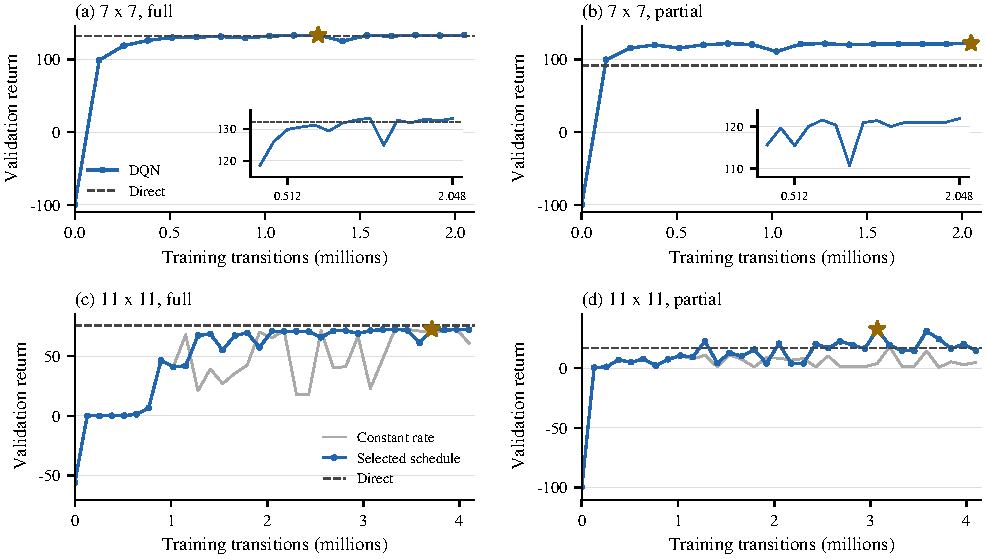
\includegraphics[width=\textwidth]{figures/native_learning.pdf}
\caption{Original-task learning on 100 fixed validation episodes. Dashed lines show Direct; stars mark submitted checkpoints. The $7\times7$ insets zoom into late learning with narrower vertical scales. On $11\times11$, schedule C is compared with constant-rate A; their initial experience is shared. All recorded evaluations along these trajectories are shown.}
\label{fig:native}
\end{figure*}

\subsection{Why extend training and reduce the learning rate?}
The smaller boards learn useful behaviour early; the larger boards improve slowly and fluctuate. More experience may help, or updates may be too large to refine a useful policy. We test these possibilities by extending training and comparing learning-rate schedules at equal budgets, holding other settings fixed.

All configurations receive 2.048 million transitions; $11\times11$ extends to 4.096 million. Schedule A keeps $10^{-4}$; B halves it to $5\times10^{-5}$ after 1.024M; C adds a reduction to $2.5\times10^{-5}$ after 2.048M. Their last-eight validation means (A/B/C) are 67.12/68.52/70.64 in full and 6.02/6.67/19.19 in partial, selecting C in both. This criterion reduces the influence of one peak. Within the chosen schedule, the earliest maximum-return validation checkpoint is retained.

\newpage
\begin{samepage}
\subsection{How performance is measured}
We fix all random seeds to 0 and use separate streams for training, exploration, replay, validation and test.

Every 128,000 training transitions, DQN is evaluated without random exploration on 100 fixed validation episodes. Learning curves show these evaluations without smoothing, together with the heuristic under the same conditions. They measure policy performance rather than the reward collected during exploratory training.\par
\end{samepage}

After selection, each frozen policy receives 500 held-out episodes of 1,000 actions. Policies share initial conditions; later fruit placements may differ as trajectories diverge. Test results do not select schedules or checkpoints. Native return differences use paired episode IDs and normal 95\% confidence intervals, $\bar\Delta\pm1.96s_\Delta/\sqrt{500}$. Classic completion uses Wilson intervals. These quantify episode uncertainty for frozen policies; one training seed leaves training variability unmeasured.



\begin{table*}[t]
\caption{Original-task test results: means over 500 episodes of 1,000 actions. DQN is the validation-selected policy. Direct has the highest heuristic return in every configuration. Bottom: paired DQN-minus-Direct return differences and 95\% confidence intervals.}
\label{tab:native}
\centering
\begin{small}
\begin{tabular}{llrrrr}
\toprule
Board / observation & Policy & Fruits & Wall hits & Body hits & Return \\
\midrule
$7\times7$ full & Direct & 286.03 & 0.00 & 53.03 & 132.41 \\
 & DQN & 288.56 & 0.46 & 54.79 & 133.27 \\
$7\times7$ partial & Direct & 199.67 & 8.76 & 30.74 & 92.81 \\
 & DQN & 266.42 & 0.01 & 55.41 & 122.13 \\
$11\times11$ full & Direct & 160.06 & 0.00 & 22.01 & 75.63 \\
 & DQN & 160.55 & 0.07 & 41.61 & 71.95 \\
$11\times11$ partial & Direct & 36.64 & 2.86 & 5.59 & 16.92 \\
 & DQN & 68.23 & 2.63 & 4.84 & 32.88 \\
\midrule
\multicolumn{2}{l}{Return: Greedy / BFS / Direct} & \multicolumn{2}{c}{Full} & \multicolumn{2}{c}{Partial} \\
\multicolumn{2}{l}{$7\times7$} & \multicolumn{2}{c}{107.93 / 110.44 / 132.41} & \multicolumn{2}{c}{85.43 / 86.47 / 92.81} \\
\multicolumn{2}{l}{$11\times11$} & \multicolumn{2}{c}{64.80 / 64.40 / 75.63} & \multicolumn{2}{c}{16.73 / 16.48 / 16.92} \\
\midrule
\multicolumn{2}{l}{DQN--Direct: difference [95\% CI]} & \multicolumn{2}{c}{Full} & \multicolumn{2}{c}{Partial} \\
\multicolumn{2}{l}{$7\times7$} & \multicolumn{2}{c}{$+0.86\ [0.39,\,1.34]$} & \multicolumn{2}{c}{$+29.32\ [28.67,\,29.96]$} \\
\multicolumn{2}{l}{$11\times11$} & \multicolumn{2}{c}{$-3.68\ [-4.06,\,-3.29]$} & \multicolumn{2}{c}{$+15.97\ [14.92,\,17.01]$} \\
\bottomrule
\end{tabular}
\end{small}
\end{table*}

\newpage
\section{What explains performance in the original task?}
\subsection{Full observation: pursuit is already a strong baseline}
On the smaller full board, DQN is competitive with Direct: returns are 133.27 and 132.41 (Table~\ref{tab:native}). Its +0.86 difference is small despite a positive episode-level confidence interval. DQN collects slightly more fruit and makes slightly more contacts. Direct reaches each fruit in minimum Manhattan time, but routes change the empty cells available for later placements. Averaging head-to-fruit Manhattan distance over every eligible spawn cell gives 3.4942 for Direct and 3.4564 for DQN on their recorded states. This measured geometric advantage helps explain the result without establishing deliberate control of fruit placement.

On the larger full board, DQN collects about as many fruits as Direct but makes nearly twice as many body contacts, explaining its lower return. Extra training helps, yet schedule C's selected test policy does not outperform constant-rate A. We retain C because validation chose it before test. Further controlled tuning could reduce unnecessary contacts; the present evidence does not show that closing this gap requires memory.



\subsection{Partial observation: learning improves the search}
Partial DQN collects about 266 versus 200 fruits for Direct on $7\times7$, and 68 versus 37 on $11\times11$. Extra collection outweighs more body contacts on the smaller board; on the larger board, collision counts also improve. More fruit within the horizon explains most of the return gain.

\begin{samepage}
We measure the time until an initially hidden fruit is first visible, using identical starting boards before later placements can diverge. DQN discovers it substantially sooner on both sizes (Table~\ref{tab:search}). For collected fruits, actions after first sighting exceed the Manhattan distance at that sighting by almost zero on the smaller board and 0.68 on the larger one. The advantage therefore reflects discovery, with little scope for faster pursuit.\par
\end{samepage}

\begin{table}[ht]
\caption{Mean actions until the initial fruit becomes visible, on the same initially hidden test starts. Failures count as 1,000 actions.}
\label{tab:search}
\centering
\begin{small}
\begin{tabular}{lrrr}
\toprule
Board & Hidden starts & Direct & DQN \\
\midrule
$7\times7$ & 220 & 7.43 & 2.02 \\
$11\times11$ & 384 & 52.15 & 10.04 \\
\bottomrule
\end{tabular}
\end{small}
\end{table}

\begin{figure*}[t]
\centering
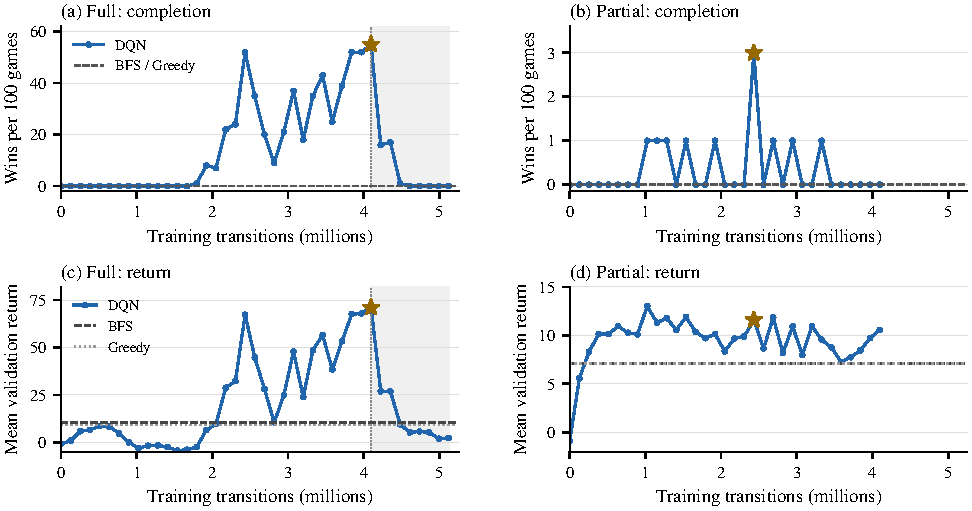
\includegraphics[width=\textwidth]{figures/classic_learning.pdf}
\caption{Classic learning on 100 fixed validation games. Stars mark the selected policies; horizontal lines show heuristic performance. Top: wins, with different scales to reveal rare partial successes. Bottom: mean undiscounted return. The shaded full-view segment continues training with unchanged settings beyond 4.096 million transitions; partial training ends there. This continuation reveals deterioration that is hidden by reporting only the selected policy.}
\label{fig:classic}
\end{figure*}

An earlier $11\times11$ partial policy collected no fruit in 247 of 500 test episodes and never saw the initial fruit in those failures. The selected policy collects fruit in every episode. Longer constant-rate training remained below Direct; schedule C surpassed it with the same reactive architecture. Its learning still fluctuates, and the final checkpoint is much weaker than the selected one (Figure~\ref{fig:native}).

This establishes better discovery than the tested random-search heuristics. Systematic coverage would provide a stronger comparison. The evidence does not identify a particular planning strategy or imply that the network has memory.



\section{Classic Snake: can collection become completion?}
\subsection{Why introduce a second task?}
The original reward can favour body cuts, avoiding part of Snake's usual survival challenge. Classic asks whether DQN can instead grow a snake that fills the board when collisions are fatal. These are new agents trained from scratch for a separate task; the original policies are not transferred.

Classic uses a $7\times7$ board, a $5\times5$ interior and initial length three. Wall or body contact ends the game; moving into the tail cell is allowed when the tail vacates on a non-fruit move. Filling all 25 interior cells wins. Fruit gives $+1$, death gives $-1$, and each action costs 0.001. A $+100$ completion bonus makes winning a strong incentive, while the step cost discourages unproductive movement. These choices express the new objective; the original and classic returns are consequently not directly comparable.

The spatial input is unchanged. Heading replaces remaining time so the input identifies the current direction of motion. Reversing direction is excluded for every policy because it moves straight into the neck; other fatal moves remain available. Greedy and BFS keep their previous rules under this restriction, falling back to a random non-reversing move when blocked. Direct is omitted because deliberately cutting through the body would now end the game.

\newpage
\subsection{Training and selecting for completion}
Both observation regimes initially train for 4.096 million transitions with the same basic DQN settings. We keep $\gamma=1$ so that the completion bonus is not reduced merely because a win takes longer. Exploration falls to 0.01 by 0.512 million transitions.

Training resets after 1,000 actions or 250 fruit-free actions to redirect collection from unproductive games. At these cutoffs, the target includes the actual next observation's value; death and victory remove it \citep[Sec.~3]{pardo2018timelimits}. Bootstrapping avoids treating a cutoff as death, but cannot supply experience beyond the reset. These limits may reduce exposure to slow successful trajectories; their effect was not isolated. Evaluation allows 5,000 actions without the fruit-free cutoff, revealing persistent failure to finish.

Selection prioritizes validation wins, then mean fruits, retaining the earlier exact tie. The highest-return partial checkpoint wins once in 100 games; the selected checkpoint wins three times despite lower return. This follows the completion goal. Selected full (4.096M) and partial (2.432M) policies each receive 500 held-out test games.

\newpage
\begin{samepage}
\subsection{Useful collection does not guarantee completion}
Full DQN wins 283 of 500 test games, versus one BFS win and two Greedy wins. Partial DQN collects more fruit than either heuristic but wins only four games (Table~\ref{tab:classic}). DQN completion is 56.6\% full (95\% Wilson interval 52.2--60.9\%) and 0.8\% partial (0.31--2.04\%): useful partial collection rarely reaches the objective.\par
\end{samepage}

\begin{table}[ht]
\caption{Classic test outcomes on 500 games per row. Fruits are means; all other entries count games. Deaths combine wall and body collisions.}
\label{tab:classic}
\centering
\begin{small}
\begin{tabular}{llrrrr}
\toprule
View & Policy & Wins & Fruits & Deaths & Timeouts \\
\midrule
Full & BFS & 1 & 11.17 & 499 & 0 \\
 & Greedy & 2 & 10.18 & 498 & 0 \\
 & DQN & 283 & 17.14 & 170 & 47 \\
Partial & BFS & 0 & 8.40 & 500 & 0 \\
 & Greedy & 0 & 8.11 & 500 & 0 \\
 & DQN & 4 & 12.29 & 154 & 342 \\
\bottomrule
\end{tabular}
\end{small}
\end{table}

\begin{samepage}
All DQN timeouts repeat a physical state: the same ordered body, heading and fruit. A deterministic policy without a changing clock then repeats its actions indefinitely. These cycles occur in 47 full games and 342 partial games, explaining much of partial DQN's failure to finish. Detection is passive: it changes neither actions nor stopping rules.\par
\end{samepage}

\begin{samepage}
The learning curves help interpret these outcomes. In partial validation, fruit collection rises from 12.20 at the selected checkpoint to 14.16 at 4.096 million transitions, while wins fall from three to zero. Full training reaches 55 wins, but an unchanged continuation to 5.120 million transitions ends with zero wins in its last five evaluations (Figure~\ref{fig:classic}). The selected policies therefore show what DQN has learned at particular points, while the curves reveal difficulties in improving it through further training.\par
\end{samepage}

\subsection{Using the observed failures to guide training changes}
Sharp full-view fluctuations motivate a smaller learning rate ($5\times10^{-5}$). For partial, the final 4.096M replay contains no winning terminal transitions despite earlier successes. Protected replay retains complete winning episodes, up to 5,000 transitions, and draws eight of each 64-sample batch from them when available. This tests whether exposure to rare successes helps completion.

For full, a Watkins-style forward-view target from replay uses $\lambda=0.8$ and at most 20 steps to propagate delayed rewards. It cuts the sequence when the next recorded action is not greedy under the target network, following the trace-cutting principle of \citet[Sec.~12.10, Fig.~12.12]{sutton2018}. A separate run sets $\gamma=0.995$ to favour nearer outcomes; this also weakens distant wins. Evaluation remains undiscounted and completion-based.

Each intervention starts from the selected checkpoint and adds 1.024M transitions. Controls continue unchanged from that checkpoint; partial uses the matching historical segment. Table~\ref{tab:interventions} reports both the best new checkpoint, selected by wins then fruits, and the last four validation means.

\begin{table}[ht]
\caption{Classic continuations: wins / mean fruits on 100 validation games. ``Best new'' excludes the starting checkpoint; ``Last four'' averages the final four evaluations. Starting scores are 55 / 16.99 (full, 4.096M) and 3 / 12.20 (partial, 2.432M).}
\label{tab:interventions}
\centering
\begin{small}
\begin{tabular}{llrr}
\toprule
View & Change & Best new & Last four \\
\midrule
Full & Control & 17 / 12.52 & 0 / 8.18 \\
 & Lower LR & 49 / 15.43 & 0 / 9.12 \\
 & Watkins-style & 1 / 8.51 & 0 / 1.29 \\
 & $\gamma=0.995$ & 21 / 14.84 & 0 / 7.49 \\
Partial & Control & 1 / 14.12 & 0.25 / 13.08 \\
 & Protected replay & 0 / 13.17 & 0 / 12.09 \\
\bottomrule
\end{tabular}
\end{small}
\end{table}

Lower LR preserves more full-view wins early than the control, but none of the new checkpoints beats its starting policy under the selection criterion. Every endpoint has zero wins. These interventions do not resolve completion under the tested conditions; they neither isolate one cause nor rule out the methods more generally.

\section{Discussion and conclusions}
The evidence suggests task-specific improvements. Native full DQN needs fewer unnecessary body contacts; native partial should be tested against systematic-search heuristics. In Classic, completion and cycle counts expose failures hidden by fruit count alone. The tested continuations improve neither selected full nor selected partial completion, so further training with those settings is not an established remedy.

Observation history is a separate hypothesis worth testing: full spatial input omits body order, and partial input also hides distant cells. Recurrent Q-learning is one concrete approach \citep[``DRQN Architecture'']{hausknecht2015drqn}; its value should be judged by more completed boards and fewer cycles at a controlled budget.

Repeated validation selection may favour that fixed sample. Held-out tests and confidence intervals characterize frozen policies, not robustness across training runs. Board-size comparisons change geometry, input dimension and budget; Classic changes several rules together. These limitations prevent a unique causal explanation, but the observed distinction is clear: DQN improves hidden-fruit discovery in the original task and often completes Classic in full view, while partial completion remains rare.

\clearpage
\bibliography{references}
\bibliographystyle{icml2021}
\end{document}
